\subsection{Comparação com as referências}
\label{sec:comparacao_referencias}

Na luz limpa, o GATv2-cascata tem erro 3-D médio \qty{1.71}{\cm} menor que o do XGBoost (\num{0.83} a \qty{2.62}{\cm}) e RMSE combinado \qty{2.30}{\cm} menor (\num{1.66} a \qty{2.95}{\cm}); contra o LightGBM, \num{1.91} e \qty{1.98}{\cm} (Figura~\ref{fig:diferenca_pareada} e Tabela~\ref{tab:referencias}). Pelas estimativas pontuais, sete dos \num{11} codificadores têm erro 3-D médio menor que o do XGBoost, mas o GATv2-cascata fica mais perto do vértice que o XGBoost em só \qty{47.6}{\percent} dos eventos: o XGBoost erra menos nos eventos mais claros, e o GATv2-cascata, nos mais escuros e na cauda, com percentil 90 do erro 3-D de \qty{51.26}{\cm} contra \qty{60.26}{\cm} (Seção~\ref{sec:onde_erro}). Nos registros das execuções, em luz com aumento, o XGBoost tem MAE médio de \qty{13.01}{\cm} e RMSE combinado de \qty{20.82}{\cm}, contra \num{13.21} e \qty{20.95}{\cm} na luz limpa.

Em relação à rede da etapa anterior \cite{vicentin2024study}, com valores obtidos em outra partição e na geometria anterior às correções, o RMSE combinado do GATv2\discretionary{-}{-}{-}cascata é \qty{10.6}{\percent} menor (\num{18.64} contra \qty{20.86}{\cm}) e o MAE médio, \qty{16.5}{\percent} menor (\num{12.63} contra \qty{15.13}{\cm}). Por eixo, no referencial dos sensores, o RMSE cai \num{4.23} e \qty{1.81}{\cm} em $x$ e $y$, e em $z$ o valor daquela rede, \qty{0.41}{\cm} maior, fica dentro do intervalo de \qty{95}{\percent} do GATv2\discretionary{-}{-}{-}cascata. Na luz limpa, os \textit{boosters} ficam a até \qty{0.24}{\cm} do RMSE combinado daquela rede, e os \num{11} codificadores, abaixo dele, entre \num{18.55} e \qty{20.64}{\cm}; para o EdgeConv, o GINE e o GINE\discretionary{-}{-}{-}cascata, como para os \textit{boosters}, o valor daquela rede fica dentro do intervalo de \qty{95}{\percent}.

\begin{table}[H]
  \centering
  \caption{Erros de teste do GATv2-cascata, do GPS e das referências, em cm, no referencial dos sensores; o baricentro tem calibração quadrática. \textsuperscript{a}RMSE por eixo citados, de outra partição (\qty{80}{\percent} e \qty{20}{\percent}) e da geometria anterior às correções \cite{vicentin2024study}, com eixos convertidos para este referencial; RMSE combinado e MAE médio calculados a partir dos valores publicados por eixo. \textsuperscript{\smash{b}}Outra simulação \cite{marinho2025apex}; larguras lidas da Figura~2 do artigo a \qty{0.26}{\cm} por \textit{pixel}, em luz detectada igual com o rendimento médio (\qty{2.9}{\MeV}) ou com o mínimo (\qty{4.9}{\MeV}) e em energia igual (\qty{10}{\MeV}); as duas larguras transversais aparecem na mesma célula, sem atribuição a $x$ e $y$; MAE não disponível.}
  \label{tab:referencias}
  \begin{tabular}{@{}l S[table-format=2.2] S[table-format=2.2] S[table-format=2.2] S[table-format=2.2] S[table-format=2.2]@{}}
\toprule
 & {RMSE $x$} & {RMSE $y$} & {RMSE $z$} & {RMSE} & {MAE} \\
Estimador & {(cm)} & {(cm)} & {(cm)} & {comb.\ (cm)} & {médio (cm)} \\
\midrule
GATv2-cascata & 20.45 & 14.35 & 20.46 & 18.64 & 12.63 \\
GPS & 20.55 & 14.29 & 20.15 & 18.55 & 12.95 \\
\midrule
XGBoost, luz limpa & 23.82 & 16.96 & 21.47 & 20.95 & 13.21 \\
LightGBM, luz limpa & 23.91 & 16.55 & 20.75 & 20.62 & 13.38 \\
Baricentro (só $z$) &  &  & 42.45 &  &  \\
\midrule
Rede densa (2024)\textsuperscript{a} & 24.68 & 16.16 & 20.87 & 20.86 & 15.13 \\
APEX, \qty{2.9}{\MeV}\textsuperscript{b} & \multicolumn{2}{c}{\num{33.1} e \num{51.3}} & 24.8 & 38.0 &  \\
APEX, \qty{4.9}{\MeV}\textsuperscript{b} & \multicolumn{2}{c}{\num{26.8} e \num{44.0}} & 19.4 & 31.8 &  \\
APEX, \qty{10}{\MeV}\textsuperscript{b} & \multicolumn{2}{c}{\num{20.8} e \num{37.3}} & 13.7 & 25.9 &  \\
\bottomrule
\end{tabular}

\end{table}

Em luz detectada igual à média do teste e com o rendimento médio, a largura combinada do APEX \cite{marinho2025apex} é de \qty{38.0}{\cm}, e o RMSE combinado do GATv2-cascata, \qty{18.64}{\cm} (\num{17.69} a \qty{19.61}{\cm}), é \qty{51.0}{\percent} menor; com o rendimento mínimo, é \qty{41.3}{\percent} menor que a largura de \qty{31.8}{\cm}, e em energia igual, \qty{28.0}{\percent} menor que a de \qty{25.9}{\cm} (Figura~\ref{fig:apex_luz}). Em $z$, contra \num{20.15} a \qty{20.46}{\cm} dos quatro melhores, o APEX tem \qty{24.8}{\cm} com o rendimento médio, acima do intervalo de \qty{95}{\percent} de cada um, e \qty{19.4}{\cm} com o mínimo, dentro dele; só em energia igual (\qty{13.7}{\cm}) é melhor. O artigo não define a largura: a \qty{4}{\MeV}, o valor do gráfico é \num{0.96} vez o desvio-padrão e \num{1.13} vez a largura gaussiana dos resíduos em $z$; uma largura gaussiana, menor que o desvio-padrão, favoreceria o APEX frente a um RMSE.

{\clubpenalty=10000 Nos mesmos eventos, o baricentro $\bar{z}$ \cite{marinho2025apex}, aqui com calibração quadrática, tem RMSE em $z$ de \qty{42.45}{\cm} (\num{39.55} a \qty{45.22}{\cm}; \qty[uncertainty-mode = separate, separate-uncertainty-units = single]{41.98 \pm 0.61}{\cm}, média e desvio-padrão em \num{30} sorteios de fótons; Figura~\ref{fig:baricentro_luz}), \num{2.07} vezes o do GATv2-cascata, e com calibração cúbica, \qty{41.86}{\cm}. Sem calibração, o baricentro tem \qty{66.59}{\cm}, deslocado em média \qty{34.08}{\cm} para a tampa mais próxima, sobretudo nos vértices a partir de $z = {}$\qty{20}{\m} (Seção~\ref{sec:onde_erro}), viés não encontrado no APEX. Dos estimadores de uma só estatística testados, o baricentro de todos os canais é o melhor (com calibração cúbica, só dos canais a mais de \qty{1}{\m} das tampas: \qty{66.95}{\cm}; canal mais claro: \qty{142.16}{\cm}).\par}

\begin{figure}[H]
  \centering
  \begin{subfigure}[t]{0.485\textwidth}
    \centering
    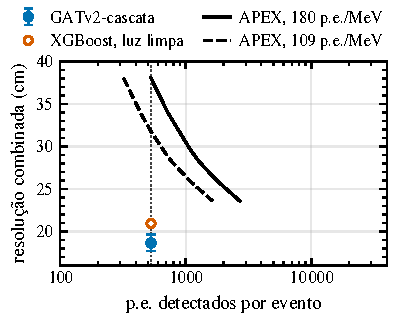
\includegraphics{figures/apex_luz.pdf}
    \caption{Largura combinada do APEX em outra simulação \cite{marinho2025apex}, com a energia convertida em fotoelétrons pelo rendimento médio (\qty{180}{\pe\per\MeV}; \qty{10}{\MeV} dão \qty{1800}{\pe}) e pelo mínimo (\qty{109}{\pe\per\MeV}), e RMSE combinado do GATv2-cascata (intervalo de \qty{95}{\percent}) e do \mbox{XGBoost} em luz limpa, na luz média do teste (\qty{530.1}{\pe}, linha pontilhada).}
    \label{fig:apex_luz}
  \end{subfigure}\hfill
  \begin{subfigure}[t]{0.485\textwidth}
    \centering
    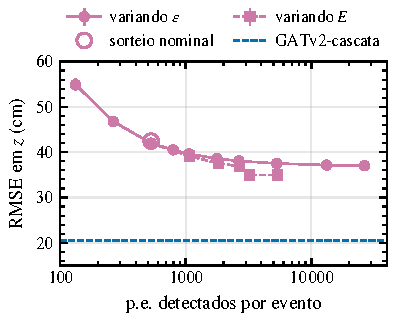
\includegraphics{figures/baricentro_luz.pdf}
    \caption{RMSE em $z$ do baricentro com calibração quadrática no teste, ao variar a eficiência $\varepsilon$ de \num{0.005} a \num{1}, com $E$ fixa em \qty{10}{\MeV}, ou a energia $E$ de \num{10} a \qty{100}{\MeV}, com $\varepsilon$ fixa em \num{0.02}: média de \num{30} sorteios de fótons e desvio-padrão (barras, menores que os marcadores, exceto em $\varepsilon = {}$\num{0.005}); círculo vazado: sorteio nominal, usado no treino e no teste dos modelos; linha horizontal: GATv2\discretionary{-}{-}{-}cascata, avaliado só nesse sorteio.}
    \label{fig:baricentro_luz}
  \end{subfigure}
  \caption{Resolução, em função da luz detectada por evento, dos estimadores analíticos e, só na luz do teste, dos modelos: (a) combinada nos três eixos; (b) em $z$.}
  \label{fig:par_luz_referencias}
\end{figure}
